\documentclass[12pt]{article}
\usepackage{graphicx}
\usepackage[margin=30mm, paper = a4paper]{geometry}
\usepackage{minted}
\usepackage{multicol}
% \usepackage[english]{babel}

\title{Basic MySQL Operations}
\author{Md Tajim An Noor}
\date{}

\begin{document}
\vspace*{\fill}
\begin{center}

    \emph{Heaven's Light is Our Guide} \\
    \textbf{Rajshahi University of Engineering and Technology} \\

    \begin{figure}[h]
        \centering
        
\includegraphics[scale=.34]{images/RUET_logo.png}
        \label{fig:ruet_logo}
    \end{figure}
    \vspace{5mm}

    \textbf{Course Code}\\
    ECE 2216\\
    \vspace{3mm}
    \textbf{Course Title}\\
    Database Systems Sessional

    \vspace{5mm}
    \textbf{Experiment Date:} October 15, 2023,\\
    \textbf{Submission Date:} November 5, 2023\\

    \vspace{5mm}
    \textbf{Lab Report 3:} Creating a database and doing operations on it using SQL\\

    \vspace{15mm}

    \begin{tabular}{c|c}
        \textbf{Submitted to} & \textbf{Submitted by} \\
        Md. Robiul Islam      & Md. Tajim An Noor     \\
        Assistant Professor   & Roll: 2010025         \\
        Dept of ECE, Ruet     &                       \\
    \end{tabular}

\end{center}
\vspace*{\fill}

\pagebreak

\tableofcontents

\maketitle

\section{Tools Used}
\begin{itemize}
    \item MySQL
    \item VS Code - as an IDE to use SQL
    \item MacTeX -\LaTeX  compiler
    \item VS Code with LaTeX workshop extension as a text editor
\end{itemize}


\section{Process}

\subsection{SQL Codes:}
\inputminted[breaklines]{SQL}{codes/Product.session.sql}

\subsection{Output}
\begin{figure}[!ht]
    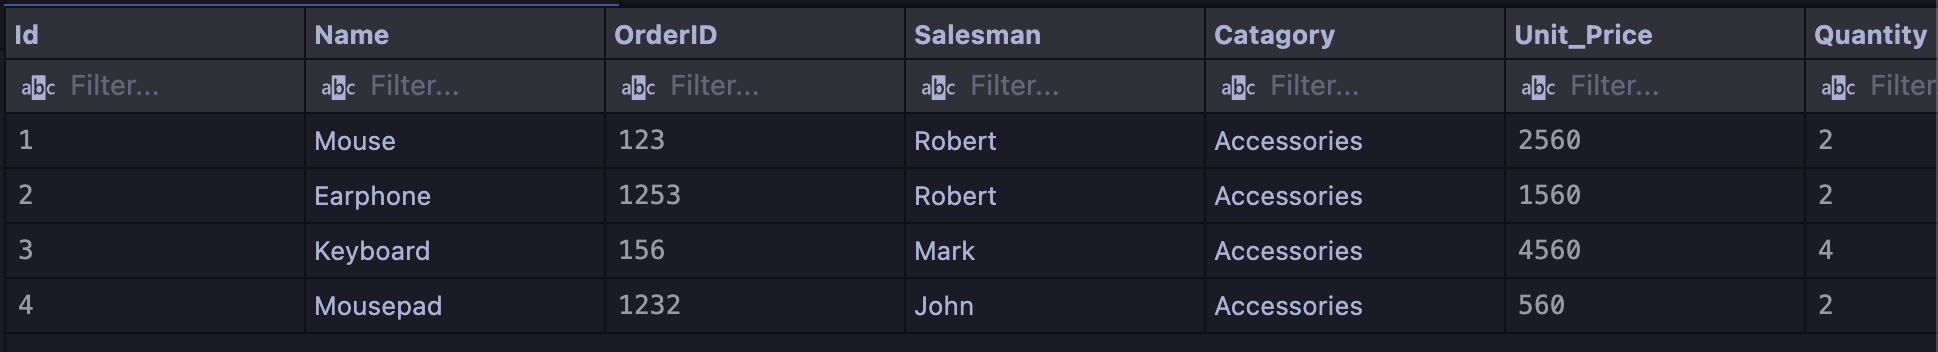
\includegraphics[width=\linewidth]{images/table.png}
    \caption{Table, ProductInfo, created using the above SQL code.}
    \label{fig:table}
\end{figure}
\begin{figure}[!ht]
    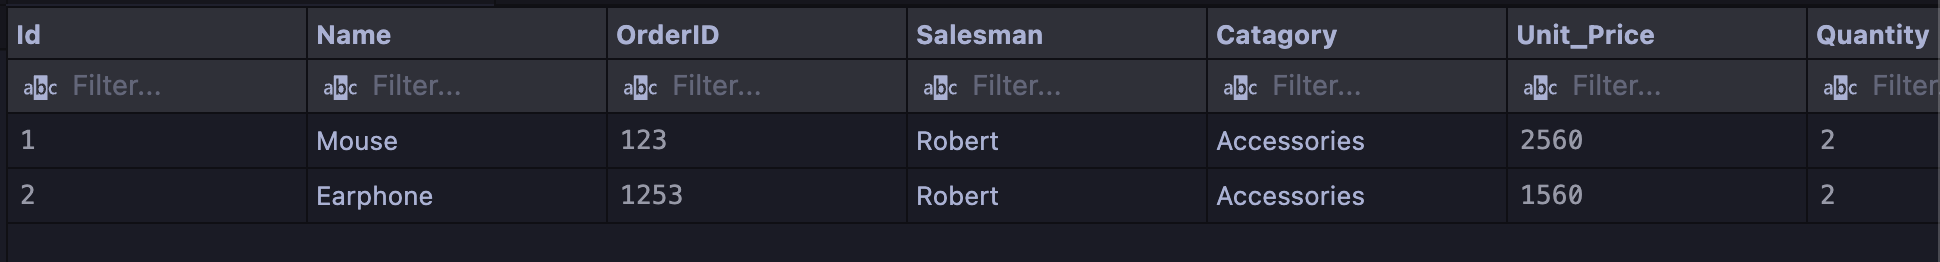
\includegraphics[width=\linewidth]{images/select.png}
    \caption{A query view from ProductInfo where Salesman is "Robert"}
    \label{fig:query}
\end{figure}


\section{Analysis}
\subsubsection{Code explanation}
First the code used:
\begin{minted}[breaklines]{SQL}
CREATE DATABASE Product;
use Product;
\end{minted}
is to first create a database named $Product$ and then by the $use$ keyword, the database is select for further operations.\\
Next by using the following code, a table in the previous database is created.
\begin{minted}[breaklines]{SQL}
CREATE TABLE
ProductInfo (
    Id int not null auto_increment primary key,
    Name varchar(30),
    OrderID int,
    Salesman varchar(20),
    Catagory varchar(20),
    Unit_Price int,
    Quantity int
)
\end{minted}
After that, insertion in the database is done using the INSERT INTO SQL:
\begin{minted}[breaklines]{SQL}
INSERT INTO
ProductProductInfo (
    Name,
    OrderID,
    Salesman,
    Catagory,
    Unit_Price,
    Quantity
)
VALUES
('Mouse', 123, 'Robert', 'Accessories', 2560.00, 3)
\end{minted}
Lastly, to view selected data in a table, the SELECT code is used:
\begin{minted}[breaklines]{SQL}
SELECT
*
FROM
Product.ProductInfo
where
Salesman = 'Robert'
\end{minted}

\section{Discussion}
Int this SQL code the Id column is kept as a primary key, and when it was initialised, AUTO\_INCREMENT was used. As such, when inserting records, no Id was provided.\\
There are some other basic operations on SQL, like DROP which removes the database. It was not included here. Some other codes like UPDATE, ALTER TABLE was also used but not shown here. I also ran some experiments with various codes to get a grasp on the SQL. It's easier than it looks. Also, the codes being not case-sensitive, makes it far easier to avoid syntax errors.

% \bibliographystyle{IEEEtran}
% \bibliography{ref}
\end{document}